
%PREAMBLE
%%%%%%%%%%%%%%%%%%%%%%%%%%%%%%%%%%%%%%%%%%%%%%%%%%%%%%%

\documentclass[titlepage,norsk]{article}
\usepackage{babel,graphicx,amsmath}
\usepackage[utf8]{inputenc}
\usepackage[margin=1.0in]{geometry}

\title{IT3708 - Evolving Spiking-Neuron Parameters}
\author{Odd Andreas Sørsæther \and Andreas Hagen}

%%%%%%%%%%%%%%%%%%%%%%%%%%%%%%%%%%%%%%%%%%%%%%%%%%%%%%%

\begin{document}
\maketitle


\section{System overview}

\paragraph{Our implementation is written in Java. Modularity is handled through ample use of interfaces.}


\subsection{The Spiking Neuron Problem}

\paragraph{
The heart of this assignment is the class SpikingNeuronProblem which implements the interface IProblem which remains unchanged. The most important attributes are shown in the class diagram below and are BIT\_LENGTH and ISDM. The ISDM is the distance metric and a description of this interface is given in a later section. The BIT\_LENGTH attribute is the number of bits used to encode the variables a,b,c,d and k in the Izhikevich model. The higher this number, the more decimals can be represented, and the less likely it is that mutations will introduce large changes in the resulting spike train. Through experimentation with the values for the different variables we discovered that the model is extremely sensitive to small changes. Changing the variable by just a small amount can result in a dramatic change in the resulting spike train. In our implementation, we opted for experimenting with values between 15 and 20 bits.
}

\begin{figure}
\centering
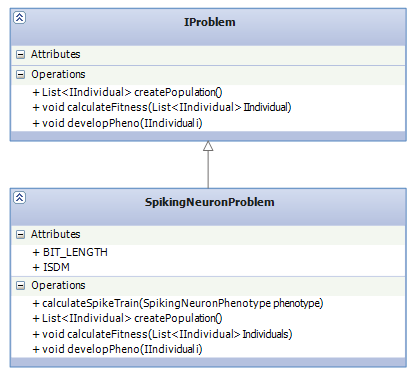
\includegraphics{SpikingNeuronProblem_UML.png}
\caption{UML diagram describing the SpikingNeuronProblem class}
\label{fig:awesome_image}
\end{figure}

\subsection{Spiketrain Distance Metrics}

\paragraph{
The three provided spike distance metrics all implement the interface ISDM (Interface Spike Distance Metric). An SDM is only required to implement the method calculateDistance which takes in two single dimensional arrays that represent the voltage levels of  two different spike-trains where the value at index i represents the voltage level at timestep t+1. The method calculates the distance according to the formulas given and returns a double representing how like each other the two spike trains are. The lower the value, the more they are seen as similar. 
}

\begin{figure}
\centering
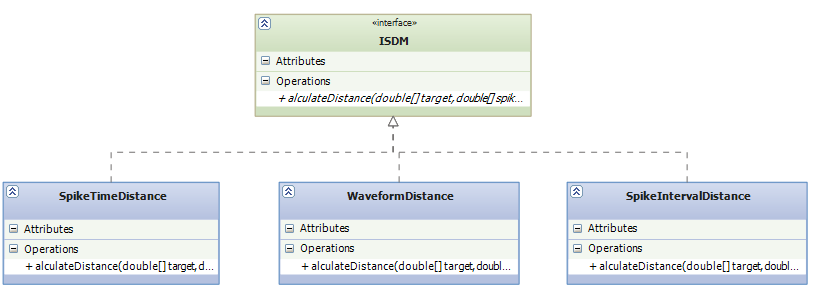
\includegraphics[scale=0.75]{ISDM.png}
\caption{UML diagram describing the ISDM}
\label{fig:awesome_image}
\end{figure}

\subsection{Fitness Function}

\paragraph{
The method calculateFitness calculates fitness for all individuals by first calculating a metric for how dissimilar the phenotype’s spike train is to the target. The largest distance calculated is seen as the worst fitness and is given the value 0. All other fitness values are computed as a percentage of this using \eqref{fitness} This means that the fitness function is relative and this entails that a fitness value is not strictly comparable between runs. We have also impemented an optional logarithmic fitness calculation. If logarithmic fitness is chosen, the fitness is calculated using \eqref{logfitness} which causes individuals that have a high distance value to have less impact on the fitness scale.
This means that the fitness function is relative and this entails that a fitness value is not strictly comparable between runs.
}

\begin{equation}\label{fitness}
\phi = 1.0 - \frac{ \delta +1.0}{\Delta + 1.0}
\end{equation}


\begin{equation}\label{logfitness}
\phi = 1.0 - \frac{ \log{ ( \delta +1.0 ) } }{\log { ( \Delta + 1.0) } }
\end{equation}

\subsection{Genotype representation}
\paragraph{
The genotype is represented using a very basic bit string. Its size is determined by a hard-coded bit-variable; it symbolizes how many bits is used to represent each variable. Currently our values are encoded in 15 bits, meaning the total genome length is 75.
}
%%%%%%%%%%%%%%%%%%%%%%%%%%%%%%%%%%%%%%%%%%%%%%%%%%%
%%% GRAPHS'N'SHIT
%%%%%%%%%%%%%%%%%%%%%%%%%%%%%%%%%%%%%%%%%%%%%%%%%%%
\section{Test Case Runs}

\subsection{Izzy Train 1}

\subsubsection{Waveform}

\begin{figure}[h!]
\centering
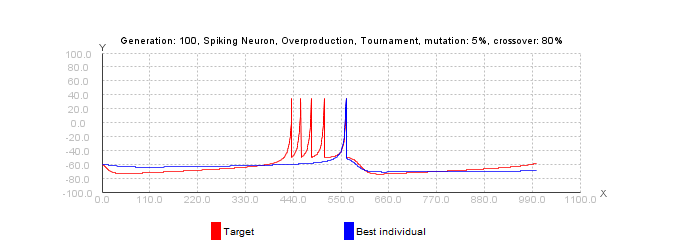
\includegraphics[scale=0.75]{izzy1wave.png}
\caption{Izzy 1 Waveform}
\label{fig:awesome_image}
\end{figure}

\begin{figure}[h!]
\centering
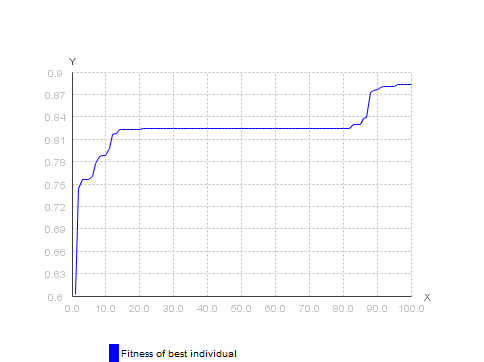
\includegraphics[scale=0.75]{izzy1waveFitness.png}
\caption{Izzy 1 Waveform Fitness Plot}
\label{fig:awesome_image}
\end{figure}

\paragraph{
Generations: 100\\
Population: 100\\
Adult Selection: Overproduction( 50 \%)\\
Selection Method: Tournament (Size: 50, best 10 \%) \\
Mutation : Variable (Initial: 5\%)\\
Crossover: 80\% 1 point split \\
Resulting fitness: 0.86 (logarithmic) \\
Values: a = 0.02, b = 0.265, c = -44.172, d = 5.108, k = 0.041 \\
}

\subparagraph{Since Waveform seems incredibly pleased with itself (high fitness) the moment it matches just a few spikes it never seems to find better solutions, or rather other good solutions may not be getting the same fitness levels.}

\subsubsection{Spike Interval Distance}

\begin{figure}[h!]
\centering
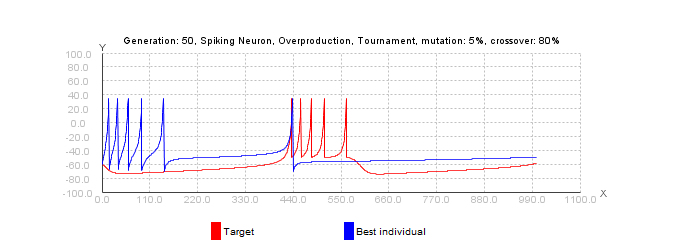
\includegraphics[scale=0.75]{izzy1interval.png}
\caption{Izzy 1 Spike Interval Distance}
\label{fig:awesome_image}
\end{figure}

\begin{figure}[h!]
\centering
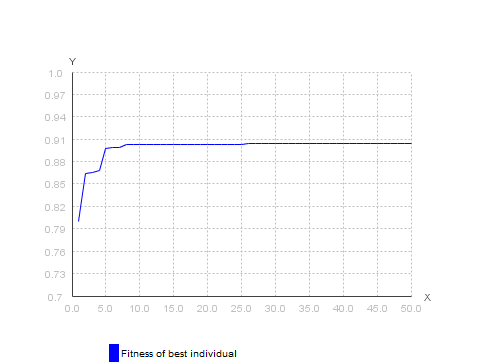
\includegraphics[scale=0.75]{izzy1intervalFitness.png}
\caption{Izzy 1 Spike Interval Fitness Plot}
\label{fig:awesome_image}
\end{figure}

\paragraph{
Generations: 100\\
Population: 100\\
Adult Selection: Overproduction( 50 \%)\\
Selection Method: Tournament (Size: 50, best 10 \%) \\
Mutation : Variable (Initial: 5\%)\\
Crossover: 80\% 1 point split \\
Resulting fitness: 0.90 (logarithmic) \\
 A: 0,002, B: 0,231, C: -74,400, D: 7,166, K: 0,054 \\
}

\subparagraph{This plot is symptomatic for Spike Interval on this problem, it tends to find the correct shape and then struggles to position it correctly along the time steps.}

\subsubsection{Spike Time  Distance}

\begin{figure}[h!]
\centering
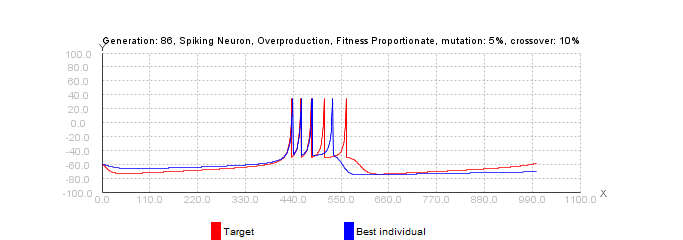
\includegraphics[scale=0.75]{izzy1spike.png}
\caption{Izzy 1 Spike Time Distance}
\label{fig:awesome_image}
\end{figure}

\begin{figure}[h!]
\centering
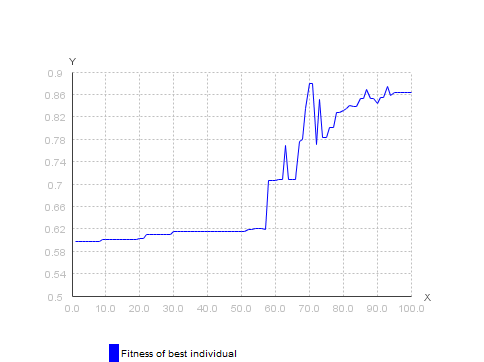
\includegraphics[scale=0.75]{izzy1spikeFitness.png}
\caption{Izzy 1 Spike Time Fitness Plot}
\label{fig:awesome_image}
\end{figure}

\paragraph{
Generations: 100\\
Population size: 100\\
Adult selection: Overproduction (50 \%) \\
Selection method: Fitness proportionate\\
Mutation: Variable,(Initial:  5\% )\\
Crossover: 80\%, 1 point split \\
Resulting fitness: 0.85 (logarithmic) \\
A: 0,007, B: 0,172, C: -47,279, D: 2,821, K: 0,041  \\
}

\subparagraph{The spike time distance is able to match up the spikes closely, but misses on the number of spikes
}
%%%%%%%%%%%%%%%%%%%%%%%%%%%%%%%%%%%%%%%%%%%%%%%%%%%%%%
\subsection{Izzy Train 2}

\subsubsection{Waveform}

\begin{figure}[h!]
\centering
\includegraphics[scale=0.75]{izzy2wave.png}
\caption{Izzy2 Waveform}
\label{fig:awesome_image}
\end{figure}

\begin{figure}[h!]
\centering
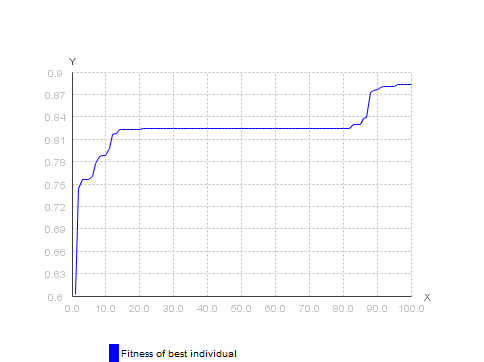
\includegraphics[scale=0.75]{izzy1waveFitness.png}
\caption{Izzy 2 Waveform Fitness Plot}
\label{fig:awesome_image}
\end{figure}

\paragraph{
Generations: 100\\
Population: 200\\
Adult Selection: Full Generational Replacement\\
Selection Method: Tournament (Size: 10, best 30 \%) \\
Mutation : 1+%\\
Crossover: 10\% 1 point split \\
Resulting fitness: 0.83 (logarithmic) \\
 A: 0,003, B: 0,089, C: -50,476, D: 5,829, K: 0,052 \\
}

\subparagraph{Since Waveform seems incredibly pleased with itself (high fitness) the moment it matches just a few spikes it never seems to find better solutions, or rather other good solutions may not be getting the same fitness levels.}

\subsubsection{Spike Interval Distance}

\begin{figure}[h!]
\centering
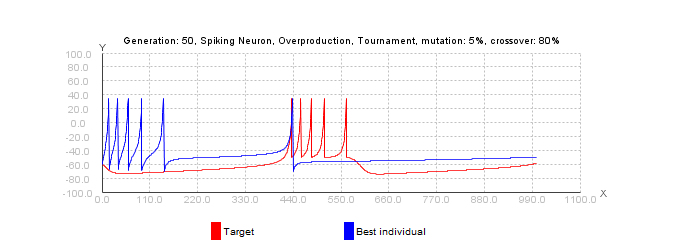
\includegraphics[scale=0.75]{izzy1interval.png}
\caption{Izzy 1 Spike Interval Distance}
\label{fig:awesome_image}
\end{figure}

\begin{figure}[h!]
\centering
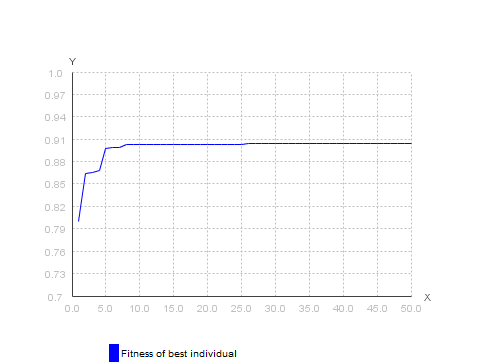
\includegraphics[scale=0.75]{izzy1intervalFitness.png}
\caption{Izzy 1 Spike Interval Fitness Plot}
\label{fig:awesome_image}
\end{figure}

\paragraph{
Generations: 100\\
Population size: 100\\
Adult selection: Generational Mixing (20 adult spots) \\
Selection method: Fitness proportionate\\
Mutation:  5\% )\\
Crossover: 80\%, 1 point split \\
Resulting fitness: 0.82 (logarithmic) \\
A: 0,017, B: 0,265, C: -69,485, D: 9,914, K: 0,072 \\
}

\subparagraph{This plot is symptomatic for Spike Interval on this problem, it tends to find the correct shape and then struggles to position it correctly along the time steps.}

\subsubsection{Spike Time  Distance}

\begin{figure}[h!]
\centering
\includegraphics[scale=0.75]{izzy2spike.png}
\caption{Izzy 2 Spike Time Distance}
\label{fig:awesome_image}
\end{figure}

\begin{figure}[h!]
\centering
\includegraphics[scale=0.75]{izzy2spikeFitness.png}
\caption{Izzy 2 Spike Time Fitness Plot}
\label{fig:awesome_image}
\end{figure}

\paragraph{
Generations: 100\\
Population size: 100\\
Adult selection: Generational Mixing (20 adult spots) \\
Selection method: Fitness proportionate\\
Mutation:  5\% )\\
Crossover: 80\%, 1 point split \\
Resulting fitness: 0.87 (logarithmic) \\
A: 0,019, B: 0,281, C: -68,388, D: 4,464, K: 0,047  \\
}

\subparagraph{Here we see behavour that we would expect of spike interval, not spike time, where the spikes are evenly distributed, but not in the correct position}


%%%%%%%%%%%%%%%%%%%%%%%%%%%%%%%%%%%%%%%%%%%%%%%%%%%%
\subsection{Izzy Train 3}

\subsubsection{Waveform}

\begin{figure}[h!]
\centering
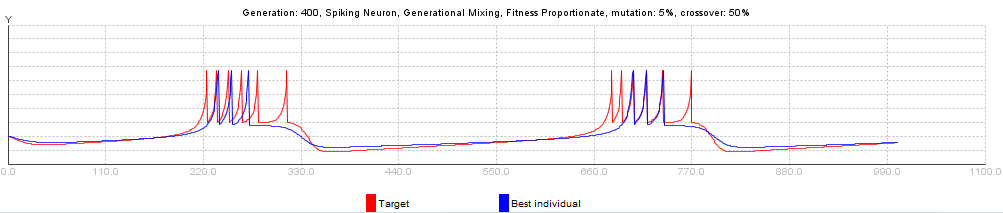
\includegraphics[scale=0.75]{izzy3wave.png}
\caption{Izzy 3 Waveform}
\label{fig:awesome_image}
\end{figure}

\begin{figure}[h!]
\centering
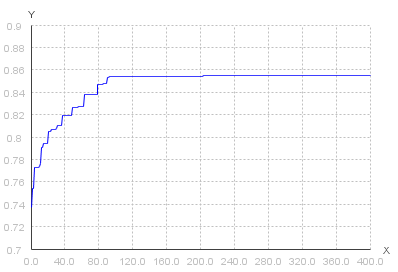
\includegraphics[scale=0.75]{izzy3waveFitness.png}
\caption{Izzy 3 Waveform Fitness Plot}
\label{fig:awesome_image}
\end{figure}

\paragraph{
Generations: 400\\
Population size: 200\\
Adult selection: Generation Mix (10) \\
Selection method: Fitness Proportionate \\
Mutation: 5\% \\
Crossover: 80\%, 1 point split \\
Resulting fitness: 0.88 (logarithmic) \\
Values: a = 0.019, b = 0.14, c = -37.133, d = 5.117, k = 0.041 \\
}

\subparagraph{Since Waveform seems incredibly pleased with itself (high fitness) the moment it matches just a few spikes it never seems to find better solutions, or rather other good solutions may not be getting the same fitness levels.}

\subsubsection{Spike Interval Distance}

\begin{figure}[h!]
\centering
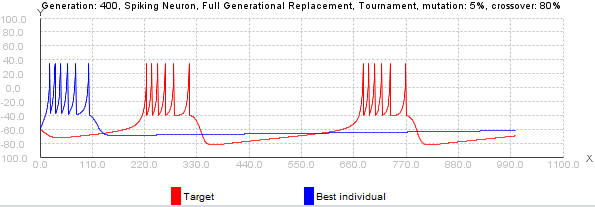
\includegraphics[scale=0.75]{izzy3interval.png}
\caption{Izzy 3 Spike Interval Distance}
\label{fig:awesome_image}
\end{figure}

\begin{figure}[h!]
\centering
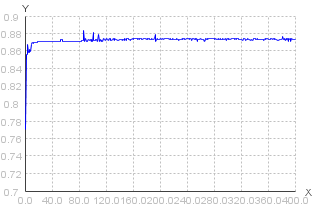
\includegraphics[scale=0.75]{izzy3intervalFitness.png}
\caption{Izzy 3 Spike Interval Fitness Plot}
\label{fig:awesome_image}
\end{figure}

\paragraph{
Generations: 400\\
Population size: 300\\
Adult selection: Full generational replacement \\
Selection method: Tournament (size: 10, best 30 \%) \\
Mutation:  Variable (initial: 5\%), 3 mutations \\
Crossover: 80\%, 1 point split \\
Resulting fitness: 0.87 (logarithmic) \\
Values: a = 0.002, b = 0.23, c = -39.129, d = 5.144, k = 0.047 \\
}

\subparagraph{This plot is symptomatic for Spike Interval on this problem, it tends to find the correct shape and then struggles to position it correctly along the time steps.}

\subsubsection{Spike Time  Distance}

\begin{figure}[h!]
\centering
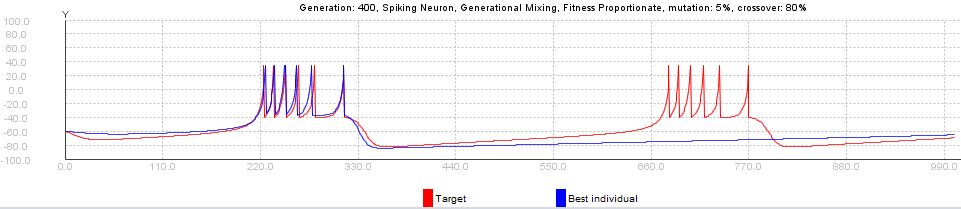
\includegraphics[scale=0.75]{izzy3spike.png}
\caption{Izzy 3 Spike Time Distance}
\label{fig:awesome_image}
\end{figure}

\begin{figure}[h!]
\centering
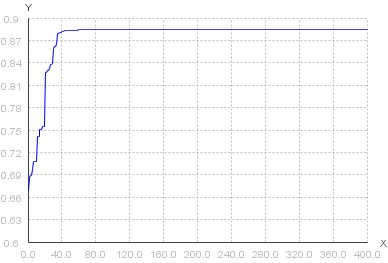
\includegraphics[scale=0.75]{izzy3spikeFitness.png}
\caption{Izzy 3 Spike Time Fitness Plot}
\label{fig:awesome_image}
\end{figure}

\paragraph{
Generations: 400\\
Population size: 200\\
Adult selection: Full generational replacement \\
Selection method: Fitness proportionate\\
Mutation: 5\% \\
Crossover: 80\%, 1 point split \\
Resulting fitness: 0.89 (logarithmic) \\
Values: a = 0.018, b = 0.261, c = -47.92, d = 1.935, k = 0.041 \\
}

\subparagraph{More commonly we get a near-perfect alignment on the first spiking group using spike time and then absolutely no other spikes, but we also tend to get this approximation, which is slightly more interesting.
}

%%%%%%%%%%%%%%%%%%%%%%%%%%%%%%%%%%%%%%%%%%%%%%%%%%%%%%

\subsection{Izzy Train 4}

\subsubsection{Waveform}

\begin{figure}[h!]
\centering
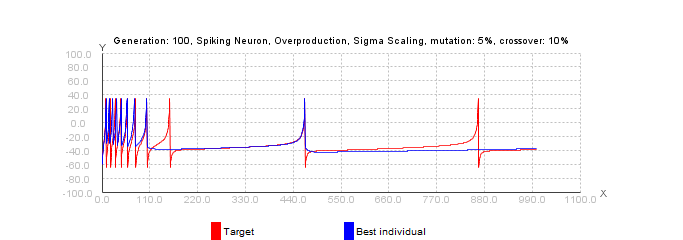
\includegraphics[scale=0.75]{izzy4wave.png}
\caption{Izzy 4 Waveform}
\label{fig:awesome_image}
\end{figure}

\begin{figure}[h!]
\centering
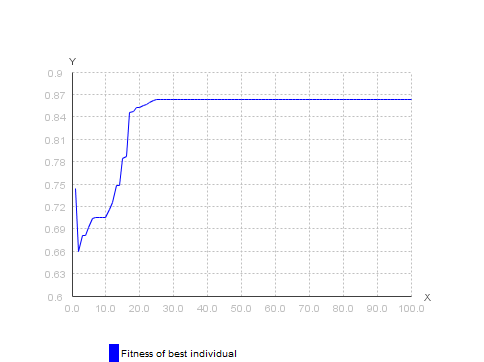
\includegraphics[scale=0.75]{izzy4waveFitness.png}
\caption{Izzy 1 Waveform Fitness Plot}
\label{fig:awesome_image}
\end{figure}

\paragraph{
Generations: 100\\
Population: 200\\
Adult Selection: Overproduction( 50 \%)\\
Selection Method: Sigma Scaling \\
Mutation : Variable (Initial: 5\%)\\
Crossover: 10\% 1 point split \\
Resulting fitness: 0.86 (logarithmic) \\
Values:A: 0,001, B: 0,173, C: -35,664, D: 8,867, K: 0,076 \\
}

\subparagraph{Another example of a common problem with this EA, the solution quickly gets stuck in local maximum and never managaes to produces an individual with a higher fitness.}

\subsubsection{Spike Interval Distance}

\begin{figure}[h!]
\centering
\includegraphics[scale=0.75]{izzy4interval.png}
\caption{Izzy 4 Spike Interval Distance}
\label{fig:awesome_image}
\end{figure}

\begin{figure}[h!]
\centering
\includegraphics[scale=0.75]{izzy4intervalFitness.png}
\caption{Izzy 4 Spike Interval Fitness Plot}
\label{fig:awesome_image}
\end{figure}

\paragraph{
Generations: 100\\
Population: 200v\\
Adult Selection: Overproduction( 50 \%)\\
Selection Method: Fitness Proportionate \\
Mutation : Variable (Initial: 5\%)\\
Crossover: 10\% 1 point split \\
Resulting fitness: 0.91 (logarithmic) \\
A: 0,010, B: 0,194, C: -34,295, D: 5,167, K: 0,044 \\
}

\subparagraph{This plot is symptomatic for Spike Interval on this problem, it tends to find the correct shape and then struggles to position it correctly along the time steps.}

\subsubsection{Spike Time  Distance}

\begin{figure}[h!]
\centering
\includegraphics[scale=0.75]{izzy4spike.png}
\caption{Izzy 4 Spike Time Distance}
\label{fig:awesome_image}
\end{figure}

\begin{figure}[h!]
\centering
\includegraphics[scale=0.75]{izzy4spikeFitness.png}
\caption{Izzy 4 Spike Time Fitness Plot}
\label{fig:awesome_image}
\end{figure}

\paragraph{
Generations: 100\\
Population size: 200\\
Adult selection: Full Generational Replacement \\
Selection method: Fitness proportionate\\
Mutation: Variable,(Initial:  5\% )\\
Crossover: 10\%, 1 point split \\
Resulting fitness: 0.88 (logarithmic) \\
 A: 0,002, B: 0,205, C: -40,516, D: 7,559, K: 0,067  \\
}

\subparagraph{In using the full generational replacement, a fairly good solution is found, but as is evident from the fitness plot, it is soon lost as small variations in the genome can produce large variations in the resulting graph
}

%%%%%%%%%%%%%%%%%%%%%%%%%%%%%%%%%%%%%%%%%%%%%%%%%%%
%%%END OF GRAPHS'N'SHIT
%%%%%%%%%%%%%%%%%%%%%%%%%%%%%%%%%%%%%%%%%%%%%%%%%%%

\section{Classification of genotype-to-phenotype mapping}
\paragraph{Since the algorithm seems to be incredibly sensitive to minor changes, having a low amount of bits dedicated to each variable (15 bits mean only 32768 possible values) can result in problems when trying to find the exact values used in the target neurons.
Another challenge comes from the fact that the five variables greatly affect the plots in different ways, meaning the EA may easily be misguided. Perhaps an approach more in the style of constraint satisfaction problems would ensure that we could make more informed searches, adjusting only one variable at a time.}

\section{Practical Implications of the Implementation}
\paragraph{Since the algorithm is designed to match target values our best guess is that a neuroscientist is able to record the voltage in a neuron or similar biological system, but is interested in determining parameters that produce the particular pattern.}
\section{Other Problem Domains}

\paragraph{
The more immediate idea we got from this particular implication is that one could create an ensemble of evolutionary algorithms using specialization-variants of this problem to find mathematical functions that fit a set of values.The algorithms could compete against each other and the EA that produces the best fitness value (best matching the plots) will be chosen. There could for instance be EAs for exponential functions, logarithmic functions, etc.
}



\end{document}